% Took this from CogSci but removed the header, sorry.
%
% Author: Matthew Turner
% Date: 2017-11-23

\documentclass[11pt,letterpaper]{article}

% \usepackage{cogsci}
\usepackage{fullpage}
\usepackage{booktabs}
\usepackage{pslatex}
\usepackage{apacite}
\usepackage{amsmath}
\usepackage{subcaption}
\usepackage[utf8]{inputenc}
\usepackage{pgfplots}
\pgfplotsset{compat=newest}
\usepgfplotslibrary{groupplots}
\usepackage{wrapfig}
% \usepackage{url}
% \usepackage{hyperref}
\usepackage{bigfoot}
\usepackage[export]{adjustbox}
\setlength\intextsep{0pt}



\usepackage{graphicx}

\usepackage{gb4e}  % linguistic examples
\noautomath

\title{Reproduction of Flache and Macy 2011 experiment two with negative valence}

\author{{\bf Matthew A.~Turner (mturner8@ucmerced.edu)}}

\begin{document}
\maketitle

We are trying to recreate the first three figures from Experiment 2 of \citeA{Flache2011},
for the cases where negative valence was allowed.

\begin{figure}
\begin{center}
  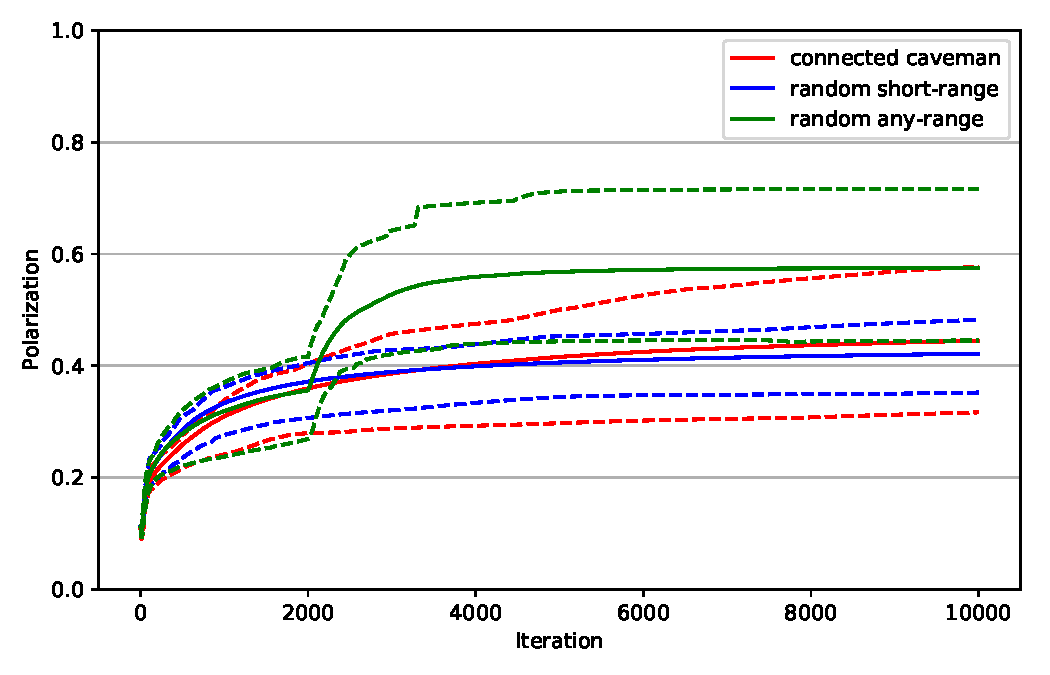
\includegraphics[width=\textwidth]{Figures/figure10b.pdf}
\end{center}
  \caption{Average of 50 trials with 25$^{\mathrm{th}}$ and 75$^{\mathrm{th}}$ percentile values
    shown at each timestep (dashed line).}
\label{fig:}
\end{figure}

\begin{figure}
\begin{center}
  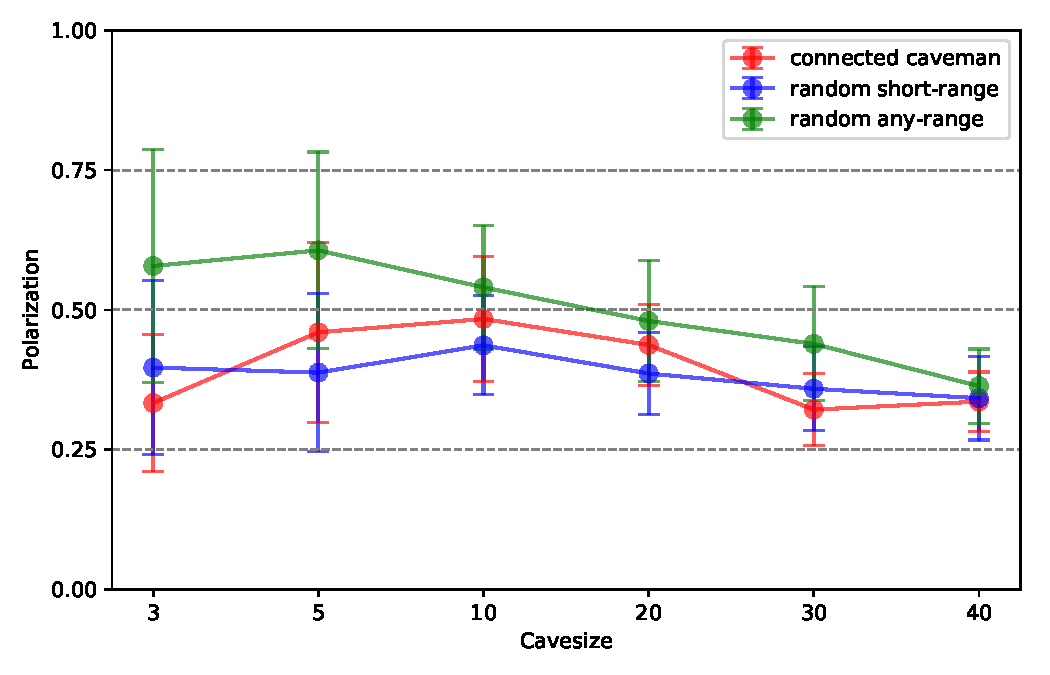
\includegraphics[width=\textwidth]{Figures/figure11b.pdf}
\end{center}
  \caption{Average of 50 trials with 25$^{\mathrm{th}}$ and 75$^{\mathrm{th}}$ percentile values
    shown at each timestep (dashed line).}
\label{fig:}
\end{figure}

\begin{figure}
\begin{center}
  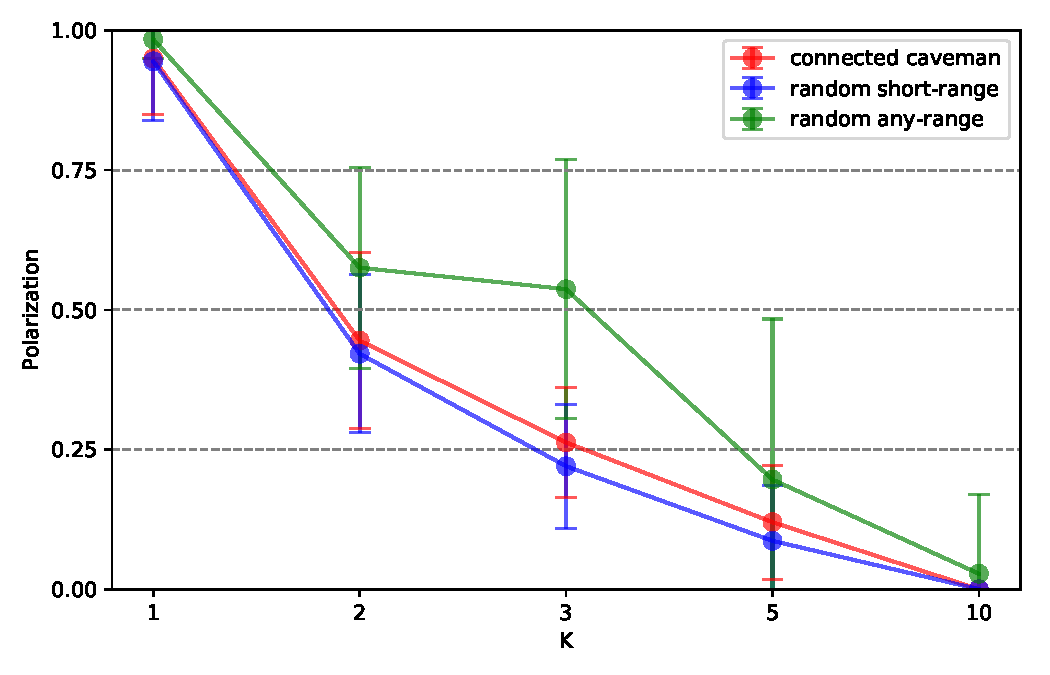
\includegraphics[width=\textwidth]{Figures/figure12b.pdf}
\end{center}
  \caption{Average of 50 trials with 25$^{\mathrm{th}}$ and 75$^{\mathrm{th}}$ percentile values
    shown at each timestep (dashed line).}
\label{fig:}
\end{figure}



\bibliographystyle{apacite}

\setlength{\bibleftmargin}{.125in}
\setlength{\bibindent}{-\bibleftmargin}

\bibliography{/Users/mt/workspace/papers/library.bib}

\end{document}
